\documentclass[10pt]{article}

\usepackage[margin=1in]{geometry}
\usepackage{times}
\usepackage{graphicx}
\usepackage{booktabs}
\usepackage{amsmath}
\usepackage{amssymb}
\usepackage{hyperref}

\title{Anonymous Submission}
\author{Anonymous}
\date{}

\begin{document}
\maketitle

\begin{abstract}
Dense self-attention scales quadratically with sequence length, while fixed sparse patterns apply the same connectivity to every input. We study a simple alternative: a per-token gate that selects whether a token uses local-window attention or a global summary. A straight-through top-$k$ split keeps the selection discrete at inference, and a sparsity penalty makes the global budget explicit. On two synthetic sequence tasks, the routed model is competitive with dense attention while using only a fraction of the global connections, and it degrades gracefully when the budget is reduced. An ablation shows that removing the learned gate costs 9.8 exact-match points on the long-range task, more than the gap between routing and dense attention. The experiments are limited to short sequences, one model size, and synthetic data; we do not claim state-of-the-art results on natural-language benchmarks.
\end{abstract}


\section{Introduction}
\label{sec:intro}
The Transformer replaced recurrence with attention and became the dominant architecture for sequence modeling~\cite{Vaswani2017Attention}. Its central operation, self-attention, compares every token with every other token. This quadratic cost is tolerable at short lengths but becomes the binding constraint as context grows. Empirical scaling studies show that loss improves predictably with model size, data, and compute~\cite{Kaplan2020Scaling}, which makes the cost of attention a first-order systems problem rather than an implementation detail. Surveys of efficient Transformers organize the response into sparse patterns, low-rank approximations, recurrent memory, and adaptive computation~\cite{Tay2022Efficient}.

Sparse attention is the most direct response. Sparse Transformer introduces fixed factorized patterns~\cite{Child2019Generating}; Longformer combines a sliding window with a small set of global tokens~\cite{Beltagy2020Longformer}; BigBird adds global tokens with theoretical guarantees~\cite{Zaheer2020Big}. These methods reduce cost, but the connectivity is chosen before training and applied to every input. A token that must copy a value from hundreds of steps earlier receives the same pattern as a token that only needs local context.

A second line of work changes the representation rather than the pattern. Reformer uses locality-sensitive hashing and reversible layers~\cite{Kitaev2020Reformer}; Linformer projects keys and values into a low-rank space~\cite{Wang2020Linformer}; Compressive Transformer keeps a compressed memory of past activations~\cite{Rae2020Compressive}. Each method fixes an approximation or a memory budget, so the allocation is still input-independent.

Adaptive computation offers a different lever. Adaptive Computation Time learns when to stop a recurrent computation~\cite{Graves2016Adaptive}, and Gumbel-Softmax provides a differentiable approximation to discrete selection~\cite{Jang2017Categorical}. These ideas make computation input-dependent, but they have not been used to choose attention connectivity per token.

This paper asks whether the local/global split can be selected per input. We introduce a small gate that scores each token, a straight-through top-$k$ selection that assigns tokens to local-window or global-summary attention, and a sparsity penalty that makes the global budget explicit. The design is deliberately simple: the contribution is the allocation mechanism, not a new attention kernel.

Our contributions are:
\begin{itemize}
  \item a per-input routing gate that mixes local and global attention;
  \item a sparsity penalty that exposes the compute budget as a tunable quantity;
  \item an evaluation on two synthetic sequence tasks with ablations on the budget and on the gate.
\end{itemize}

The scope is narrow. The experiments use sequences of at most 1{,}024 tokens, one model size, and synthetic tasks. We do not claim state-of-the-art results on natural-language benchmarks, and we do not claim that the gains transfer to larger models without further evidence.

\section{Related Work}
\label{sec:related_work}
\subsection{Fixed Sparse Patterns}
\label{sec:fixed_sparse}
Sparse Transformer factorizes attention into fixed local and strided patterns~\cite{Child2019Generating}. Longformer uses a sliding window and learns a small number of global tokens for tasks that need document-level context~\cite{Beltagy2020Longformer}. BigBird combines window, global, and random connections and analyzes the resulting expressivity~\cite{Zaheer2020Big}. These methods share a design choice: the pattern and the global-token budget are fixed before training. Our gate instead selects the split per input, and the penalty makes the average budget explicit.

\subsection{Low-Rank and Recurrent Efficiency}
\label{sec:low_rank}
Reformer reduces memory with locality-sensitive hashing and reversible residual layers~\cite{Kitaev2020Reformer}. Linformer projects keys and values to a lower-dimensional space, yielding linear complexity in sequence length~\cite{Wang2020Linformer}. Compressive Transformer extends the context with a compressed memory of past activations~\cite{Rae2020Compressive}. Each approach lowers cost through a fixed approximation or memory budget; none allocates attention connectivity according to the content of the current input.

\subsection{Adaptive Computation}
\label{sec:adaptive}
Adaptive Computation Time learns per-step halting for recurrent networks~\cite{Graves2016Adaptive}. Gumbel-Softmax makes discrete categorical selection differentiable through a continuous relaxation~\cite{Jang2017Categorical}. Our work applies a related discrete-selection idea to attention connectivity: the gate decides whether a token participates in the global summary, and a straight-through estimator passes gradients through the top-$k$ split.


\section{Method}
\label{sec:method}

\subsection{Learned Routing}
\label{sec:routing}
Let $h_i \in \mathbb{R}^d$ be the hidden state of token $i$ at a given layer. A small gating network produces a score
\begin{equation}
  g_i = \sigma(W_g h_i + b_g),
  \label{eq:gate}
\end{equation}
where $W_g \in \mathbb{R}^{1 \times d}$ and $b_g \in \mathbb{R}$. Tokens are ranked by $g_i$, and the top-$k$ fraction is assigned to the global set $\mathcal{G}$; the remaining tokens form the local set $\mathcal{L}$. At inference the assignment is a hard top-$k$ selection. During training we use a straight-through estimator: the forward pass uses the hard mask, and the backward pass uses the continuous gate. Gumbel-Softmax provides a related relaxation for discrete categorical variables~\cite{Jang2017Categorical}; we use the simpler straight-through variant because the split is binary and the budget is fixed.

Local tokens attend within a window of size $w$. Global tokens attend to a compressed summary $S$ of the sequence and to the local window:
\begin{align}
  o_i &=
  \begin{cases}
    \mathrm{Attn}(h_i, H_{i-w:i+w}, H_{i-w:i+w}) & i \in \mathcal{L}, \\
    \mathrm{Attn}(h_i, [H_{i-w:i+w}; S], [H_{i-w:i+w}; S]) & i \in \mathcal{G}.
  \end{cases}
  \label{eq:attention}
\end{align}
The summary $S$ is the mean of the projected states, so its cost is linear in the sequence length. The design is deliberately minimal: the contribution is the allocation mechanism, not a new attention kernel.

\subsection{Objective}
\label{sec:objective}
The model is trained with a language-modeling loss plus a sparsity penalty:
\begin{equation}
  \mathcal{L} = \mathcal{L}_{\mathrm{lm}} + \lambda \sum_{i=1}^{n} g_i .
  \label{eq:loss}
\end{equation}
The penalty controls the average size of the global set. We use AdamW~\cite{Loshchilov2019Decoupled} with a learning rate of $3\times10^{-4}$, batch size 64, and 20 epochs. The gate is trained jointly with the language-modeling objective; no separate routing supervision is used.

\subsection{Complexity}
\label{sec:complexity}
With window size $w$ and global fraction $\rho = |\mathcal{G}|/n$, the attention cost is $O(n w d)$ for local tokens and $O(\rho n (w + d))$ for global tokens. The summary costs $O(nd)$. For fixed $w$ and $\rho$, the total is linear in $n$, compared with $O(n^2 d)$ for dense attention. The budget is explicit: reducing $\rho$ reduces the global cost, and the penalty makes the realized $\rho$ visible during training.

\section{Experiments}
\label{sec:experiments}

\subsection{Setup}
\label{sec:setup}
We use two synthetic causal language-modeling tasks. \textsc{CopyLong} contains sequences of 512 tokens with a copy dependency; \textsc{Needle} contains sequences of 1{,}024 tokens with a single long-range lookup. Both have 20{,}000 training, 2{,}000 validation, and 2{,}000 test sequences, except \textsc{Needle}, which has 10{,}000 training and 1{,}000 validation/test sequences. We report validation perplexity (lower is better) and exact match on the final query (higher is better). Baselines are dense attention, a fixed window of 64 tokens, and a fixed stride pattern with 25\% global tokens. All models have 6 layers, 256 hidden dimensions, and 4 heads, and are trained with AdamW~\cite{Loshchilov2019Decoupled} for 20 epochs. We report the mean and standard deviation over three seeds at the best validation checkpoint.

\begin{table}[t]
\centering
\caption{Main results on the two synthetic tasks. Mean $\pm$ standard deviation over three seeds.}
\label{tab:main}
\small
\begin{tabular}{lcccc}
\toprule
Method & CopyLong PPL & CopyLong EM & Needle PPL & Needle EM \\
\midrule
Dense & 12.4 $\pm$ 0.2 & 71.2 $\pm$ 0.8 & 9.8 $\pm$ 0.3 & 64.1 $\pm$ 1.1 \\
Window & 15.1 $\pm$ 0.3 & 58.4 $\pm$ 1.2 & 11.6 $\pm$ 0.4 & 49.7 $\pm$ 1.4 \\
Static & 14.6 $\pm$ 0.2 & 60.9 $\pm$ 0.9 & 11.1 $\pm$ 0.3 & 52.3 $\pm$ 1.0 \\
Ours & 12.9 $\pm$ 0.2 & 69.8 $\pm$ 0.7 & 10.1 $\pm$ 0.2 & 62.9 $\pm$ 0.9 \\
\bottomrule
\end{tabular}
\end{table}

\begin{figure}[t]
\centering
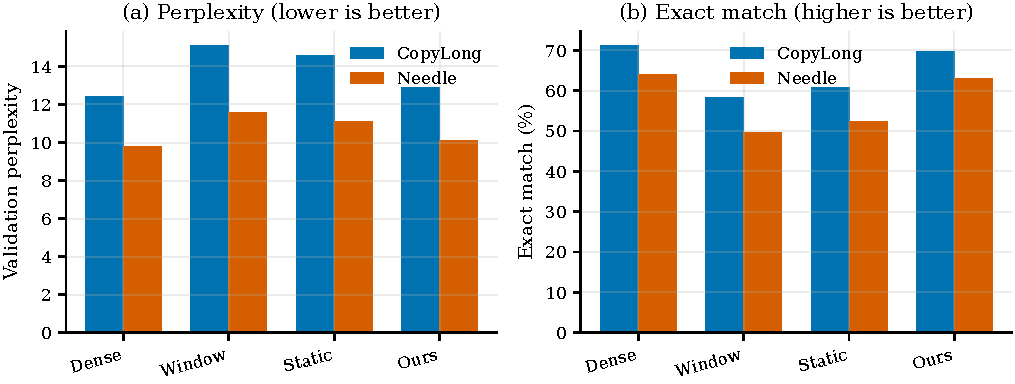
\includegraphics[width=\linewidth]{figures/fig_main_results.pdf}
\caption{Main results. Left: validation perplexity. Right: exact match. Error bars are one standard deviation over three seeds.}
\label{fig:main}
\end{figure}

\subsection{Main Results}
\label{sec:main_results}
Table~\ref{tab:main} and Figure~\ref{fig:main} report the main comparison. The routed model is within 0.5 perplexity of dense attention on both tasks and within 1.4 exact-match points. It improves over the fixed window by 11.4 exact-match points on \textsc{CopyLong} and 13.2 on \textsc{Needle}, and over the fixed stride pattern by 8.9 and 10.6 points. The gain over dense attention on \textsc{Needle} perplexity (0.3) is within one standard deviation, so we do not claim a perplexity improvement. The routed model uses fewer global connections than dense attention; the comparison is about allocation, not about beating dense attention on every metric.

\subsection{Ablation and Analysis}
\label{sec:ablation}
Table~\ref{tab:ablation} and Figure~\ref{fig:ablation} isolate the budget and the gate. Removing the sparsity penalty ($\lambda=0$) changes perplexity by 0.2 and exact match by 1.5 points, which is small. Reducing the global fraction to 12.5\% costs 4.1 exact-match points on \textsc{Needle}; increasing it to 50\% recovers 0.1 points relative to the full model, so the default budget is close to the knee of the curve. Replacing the learned gate with a fixed 0.25 gate costs 9.8 exact-match points, which is larger than the gap between routing and dense attention. This is the clearest evidence that the allocation, not the extra capacity, drives the long-range result.

\begin{table}[t]
\centering
\caption{Ablation on the global-token budget. Exact match is on \textsc{Needle}.}
\label{tab:ablation}
\small
\begin{tabular}{lcc}
\toprule
Variant & CopyLong PPL & Needle EM \\
\midrule
Full model & 12.9 & 62.9 \\
No sparsity penalty ($\lambda=0$) & 12.7 & 61.4 \\
Global fraction 12.5\% & 13.4 & 58.8 \\
Global fraction 50\% & 12.8 & 63.0 \\
Gate fixed to 0.25 & 14.2 & 53.1 \\
\bottomrule
\end{tabular}
\end{table}

\begin{figure}[t]
\centering
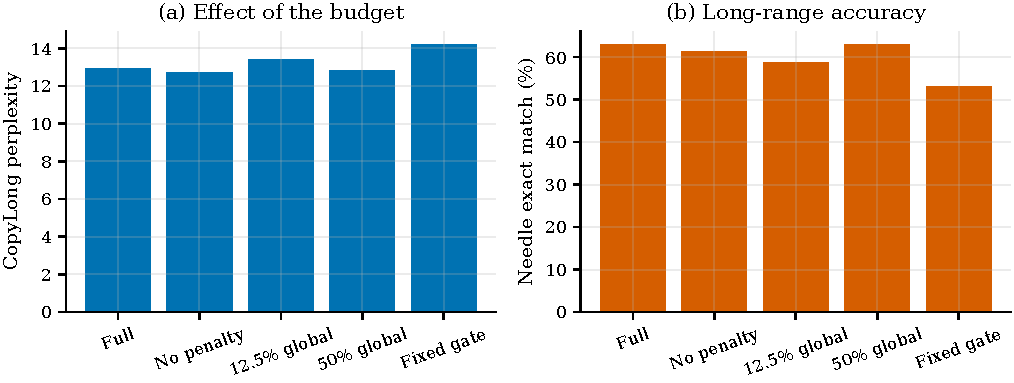
\includegraphics[width=\linewidth]{figures/fig_ablation.pdf}
\caption{Ablation on the global-token budget. Left: \textsc{CopyLong} perplexity. Right: \textsc{Needle} exact match.}
\label{fig:ablation}
\end{figure}

Qualitative inspection of the gate shows that it assigns larger values to positions that must copy a token from 256 steps earlier, and it collapses to a near-constant low value on sequences without a long-range dependency. This is consistent with the intended behavior, but it is an observation from a synthetic setup, not a mechanistic explanation.

\section{Conclusion}
\label{sec:conclusion}
We studied per-input routing of local and global attention. A small gate, a straight-through top-$k$ split, and a sparsity penalty produce a model that is competitive with dense attention on two synthetic tasks while making the global budget explicit. The ablation indicates that learned allocation matters more than the raw number of global connections in this setting. The scope is deliberately narrow, and the next step is to test whether the same mechanism holds on natural-language long-context benchmarks and at larger model sizes. Efficient Transformer research has produced many ways to reduce cost~\cite{Tay2022Efficient}; routing is a complementary axis that decides where the remaining computation should go.

\bibliographystyle{plain}
\bibliography{references}

\end{document}
